% This file is part of JTS-MM (https://github.com/paulotto/jts-mm).
% SPDX-FileCopyrightText: 2026 Paul-Otto Müller
% SPDX-License-Identifier: CC-BY-4.0

\section{Why the molars, and why the lingual side}\label{sec:mechanics}

A crown is not a cylinder. Seen along the path along which the appliance is inserted (here the
model $z$ axis), each face bulges out to a \emph{height of contour} and then recedes again toward
the gum. The region between the height of contour and the gingival margin is the
\emph{undercut}. A jaw pressing on the face above the height of contour sits on a surface that
converges occlusally, and the reaction force has an occlusal component: the part is pushed off
(\cref{fig:mech}a). The same jaw placed below the height of contour sits on a surface that
converges gingivally, and the reaction has a gingival component: the part is pulled on
(\cref{fig:mech}b). The clamping force stops being the failure mode and becomes the retention.

\begin{figure}[H]
\centering
\begin{subfigure}[t]{0.325\textwidth}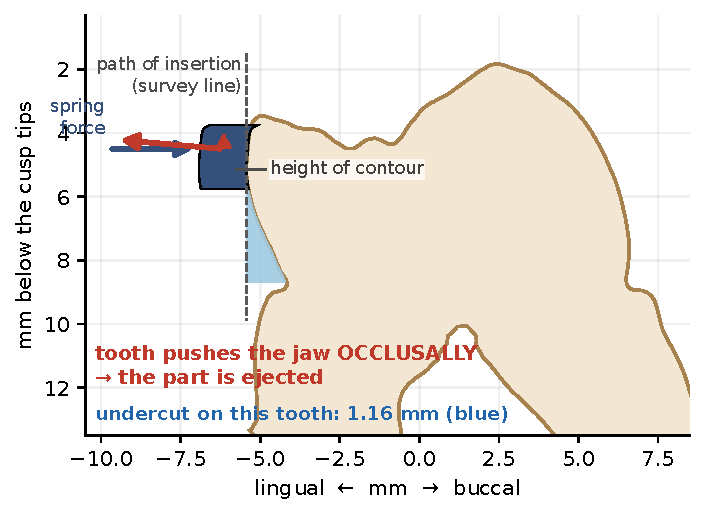
\includegraphics[width=\linewidth]{mech_eject}\caption{Jaw above the lingual height of contour of the first molar.}\end{subfigure}\hfill
\begin{subfigure}[t]{0.325\textwidth}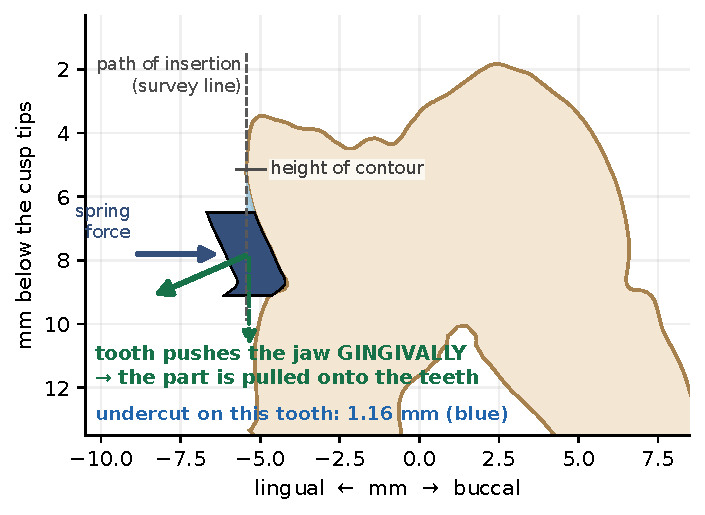
\includegraphics[width=\linewidth]{mech_seat}\caption{Same molar, jaw below it: the same spring seats the part.}\end{subfigure}\hfill
\begin{subfigure}[t]{0.325\textwidth}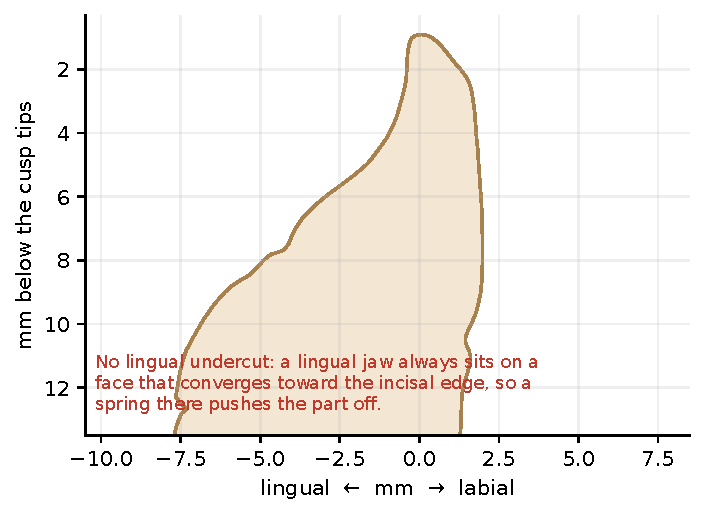
\includegraphics[width=\linewidth]{mech_incisor}\caption{Lower central incisor: the lingual face only widens toward the gum.}\end{subfigure}
\caption{Real sections through \texttt{Teeth\_02}, perpendicular to the arch. Solid arrow: force
of the tooth on the jaw; dashed: its component along the path of insertion.}
\label{fig:mech}
\end{figure}

\Cref{fig:undercut} and \cref{tab:survey} list the undercut on every tooth. Three things follow:
\begin{itemize}
\item \textbf{Molars retain lingually.} First and second molars have
\SIrange{0.3}{1.2}{\milli\metre} of lingual undercut and only \SIrange{0.03}{0.13}{\milli\metre}
buccally. The buccal jaw of any clamp is therefore a rigid \emph{reciprocal} arm that only takes
the reaction force; it cannot hold the part by itself.
\item \textbf{Incisors and canines have no lingual undercut at all.} This is the root cause of the
slipping incisor attachment, independent of how hard the screws are tightened.
\item \textbf{The numbers depend on the path of insertion.} The left/right difference is partly
the tilt of the model. Tilting the path moves undercut from one face to the other; choose it on
the subject's scan so that both molars get \SIrange{0.3}{0.5}{\milli\metre} lingually, then block
out anything deeper.
\end{itemize}

\begin{figure}[H]
\centering
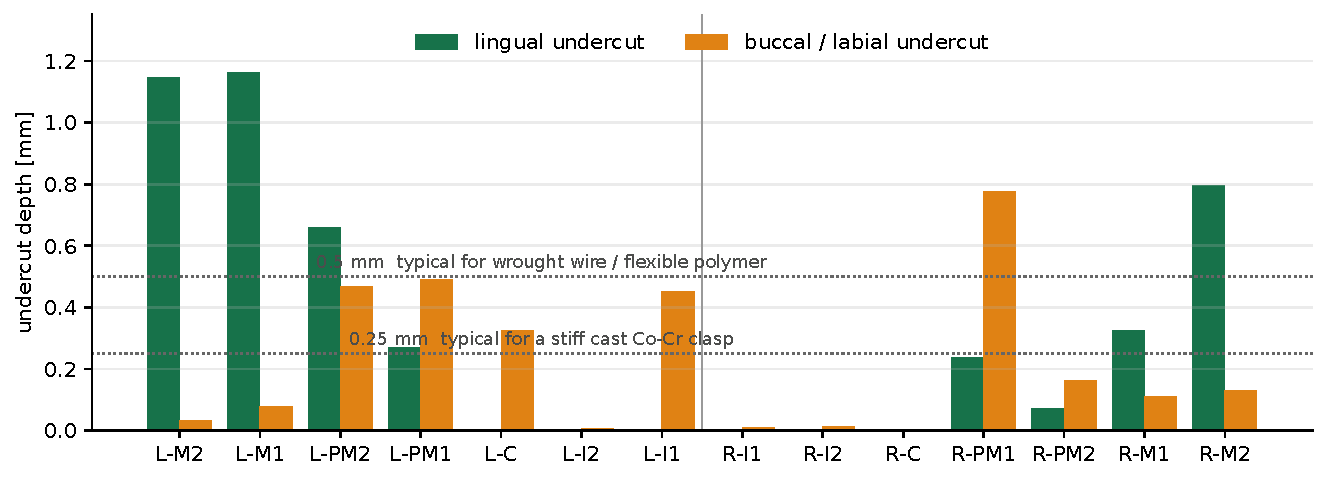
\includegraphics[width=\textwidth]{mech_undercut_bars}
\caption{Usable undercut per tooth for a vertical path of insertion. Dotted lines: typical
engagement depths used for removable-partial-denture clasps.}
\label{fig:undercut}
\end{figure}

\begin{table}[H]
\centering\small
\caption{Undercut depth in mm (output of \texttt{s03\_survey.py}).}\label{tab:survey}
\begin{tabular}{l S[table-format=1.2] S[table-format=1.2] S[table-format=1.2] S[table-format=1.2]}
\toprule
& \multicolumn{2}{c}{left} & \multicolumn{2}{c}{right}\\
\cmidrule(lr){2-3}\cmidrule(lr){4-5}
tooth & {lingual} & {buccal} & {lingual} & {buccal}\\
\midrule
\inputrows{generated/survey_table.tex}
\bottomrule
\end{tabular}
\end{table}

\paragraph{Limits of the model.} The intraoral scan closes the gaps between teeth below the
contact points, so the interproximal undercuts that Adams clasps and resin relines use in a real
mouth do not appear in these numbers. The gingiva is part of the model, so the ``gingival margin''
is where the scanned gum starts.
